\chapter{Metodología}\label{Metodología}
%Función que crea el título de capítulo y al cual se le da el nombre deseado a través de su parámetro obligatorio. Al no tener la función el “*” se escribirá también en el título del documento las palabras “Capítulo 1: …”. Además se indica, mediante la función “\label”, la correspondiente etiqueta que lleva asociada. La etiqueta sirve para que en caso de que luego se quiera hacer referencia al capítulo se haga llamando etiqueta tal que se escribiría “La información correspondiente a dicho tema se encuentra en el capítulo \ref{Int}.”

\thispagestyle{fancy}
%Función que determina que durante este capítulo se aplique el estilo Fancy.

\fancyhead[LE]{\thechapter.Metodología} 
%Función que se utiliza para indicar que en las páginas impares, aparezca en el encabezado en la parte izquierda, el número del capítulo con su correspondiente nombre.

\section{Desarrollo ágil}
Este proyecto nace de una idea tan amplia como el \textit{SSI}. No había requisitos iniciales y ni se conocía el alcance. Para poder estudiar las posibilidades tan amplias con las que se puede afrontar, se seleccionó la metodología SCRUM. Esta metodología está pensada para equipos con reuniones periódicas y \textit{sprints} de trabajo. Cada \textit{sprint} de trabajo tiene unos objetivos. Estos se comprobarán al final con una reunión.
En este caso, tras realizar un objetivo se aseguraba su funcionamiento y se comprobaban las metas. De este modo, se consigue enfocar los requisitos del proyecto al mismo tiempo que se asegura el funcionamiento global de la aplicación.
Como SCRUM es una metodología extensa y complicada, se va a introducir en este trabajo. Dicha metodología cuenta con cuatro pilares:
\begin{itemize}
    \item \textbf{Equipo SCRUM}\\
    Para poder realizar un trabajo, se necesita un motor para hacer mover las tareas.
    En el caso de este proyecto, el trabajo ha sido realizado por una sola persona. Las reuniones de control se realizaban con el director del proyecto al final de cada \textit{sprint}.
    \item \textbf{Backlog o lista de tareas}\\
    \begin{figure}[H]
        \centering
        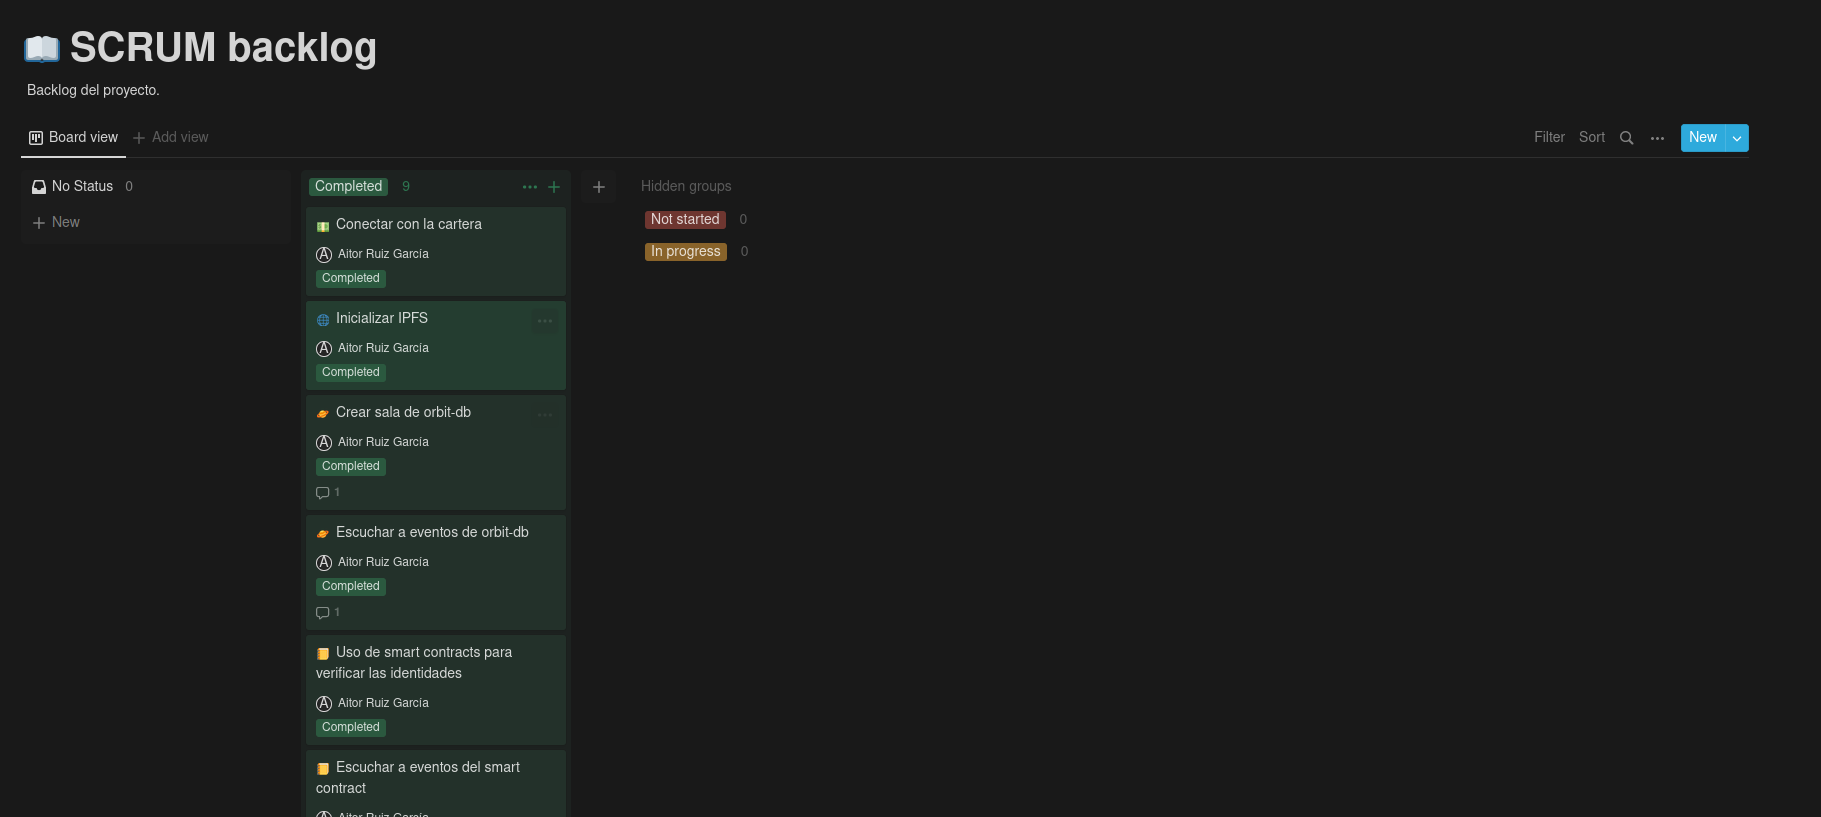
\includegraphics[width=0.8\textwidth]{Figures/Screenshot_20220601_182542.png}
        \caption{Imagen del backlog del proyecto}
        \label{fg:backlog}
    \end{figure}
    El desarrollo se ha estado controlando desde \verb|notion.so| \cite{web:notion}. Notion genera un archivo \verb|markdown|. Este fichero puede ser enriquecido con distintos \textit{widgets}. Uno de estos \textit{widgets} es una \textit{board view}. Esta inspirado en otras herramientas que permiten hacer \textit{backlogs} \ref{fg:backlog}.
    Se crearon temas que cumplían uno o varios requisitos del proyecto al mismo tiempo y que estaban relacionados entre sí. Estas tarjetas pueden ser desplazadas dependiendo del estado en el que se encuentran.
    \begin{itemize}
        \item \verb|No iniciado|
        \item \verb|En proceso|
        \item \verb|Completada|
    \end{itemize}
    Dentro de estas tarjetas se puede escribir y anotar elementos, por ejemplo: las horas invertidas en el desarrollo. Esto resulta útil para las reuniones y para el presupuesto.
    \item \textbf{\textit{Sprint}}\\
    Cuando se completa un \textit{sprint}, si se ha realizado la tarea correspondiente, la tarjeta deberá ser desplazada a \verb|completada|.
    En esta tarjeta, si se selecciona, se puede acceder a la información en su interior \ref{fg:tarjeta}.
    \begin{figure}[h!]
        \centering
        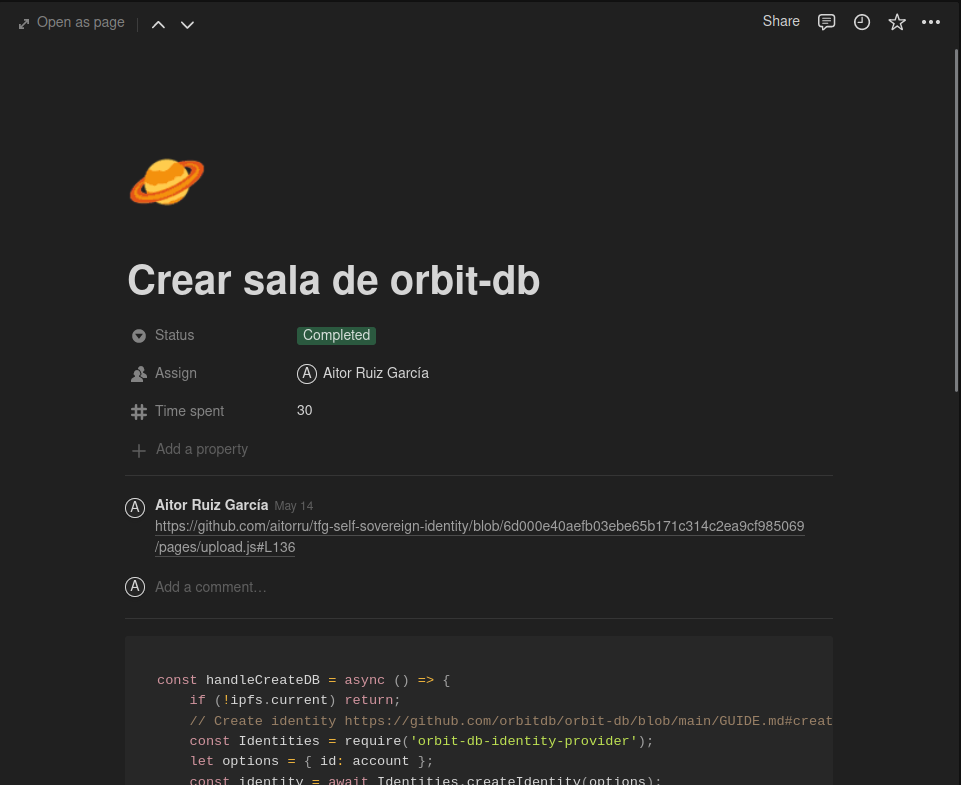
\includegraphics[width=0.7\textwidth]{Figures/Screenshot_20220601_181036.png}
        \caption{Imagen de los datos dentro de una tarjeta.}
        \label{fg:tarjeta}
    \end{figure}
    \item \textbf{Reuniones de seguimiento (bisemanales)}\\
    Para hacer las reuniones, se necesita disponer un guion donde se apuntará información útil asociados a la tarjeta. Ese conocimiento puede ser utilizado para el resto de los \textit{sprints}.
\end{itemize}
\section{Herramientas de desarrollo}
Un elemento fundamental para el desarrollo de esta aplicación ha sido \verb|Next.js| \cite{web:next.js}. Es un \textit{framework} \cite{web:framework} para generar paginas estáticas, con capacidad de utilizar SSR (renderizado de servidor \cite{web:ssr}) e ISR (renderizado estático incremental \cite{web:isr}).
En el apartado \textbf{Herramientas utilizadas}, se explicará por que se ha elegido un \textit{framework} basado en React. Aun así, solo estamos interesados en dos aspectos:
\subsection{Páginas estáticas}
Como hemos dicho anteriormente, en IPFS se pueden subir ficheros. Por lo cual podemos subir archivos \verb|.html|.
En el esquema de acceso clásico en una página, todos los usuarios acceden a un servidor centralizado \ref{fg:centralizado}.
\begin{figure}[H]
    \centering
    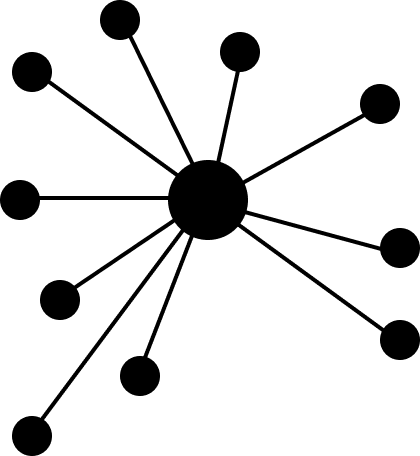
\includegraphics[width=0.5\textwidth]{Figures/Centralizado.png}
    \caption{Imagen para explicar la centralización de un servidor. \textbf{El nodo con mayor tamaño es el servidor, el resto son usuarios que quieren conectarse.}}
    \label{fg:centralizado}
\end{figure}
Una implementación que cuente con más recursos, puede tener más nodos centralizados más cerca de sus usuarios, pero eso solo se lo pueden permitir organizaciones con muchos recursos.
Cuando una página no dispone de más servidores repartidos por el mundo, solo tiene un punto de acceso. IPFS viene al rescate ya que todos los ficheros que son compartidos, son \textit{cacheados}. Haciendo que cuanto más se use un fichero, más rápido se accederá a él.
Todos los ficheros estáticos pueden ser alojados en IPFS y visitados de la siguiente manera: tomando de ejemplo la documentación de IPFS \cite{web:ipfs_whatis}, imaginemos que queremos acceder a Wikipedia \cite{web:wikipedia_main}.
El servidor de Wikipedia puede estar al otro lado del mundo o en otro planeta. Aun así, en tu cercanía, es probable que otra persona también quiera acceder a Wikipedia. Para eso, se puede buscar si alguien tiene la página en la red de IPFS.
\begin{quote}
    \verb|/ipfs/QmXoypizjW3WknFiJnKLwHCnL72vedxjQkDDP1mXWo6uco/wiki|
\end{quote}
Si se introduce este DID en el navegador, no significa nada, ya que de manera nativa un navegador no puede convertirse en un nodo de IPFS. Por eso mismo, se necesita una manera de ejecutar \verb|js-ipfs| (una librería que se explicará más adelante) para poder recibir el fichero.
Existen muchas puertas de entrada \ref{fg:ipfs_entry} e incluso se pueden crear nuevas.
\begin{figure}[H]
    \centering
    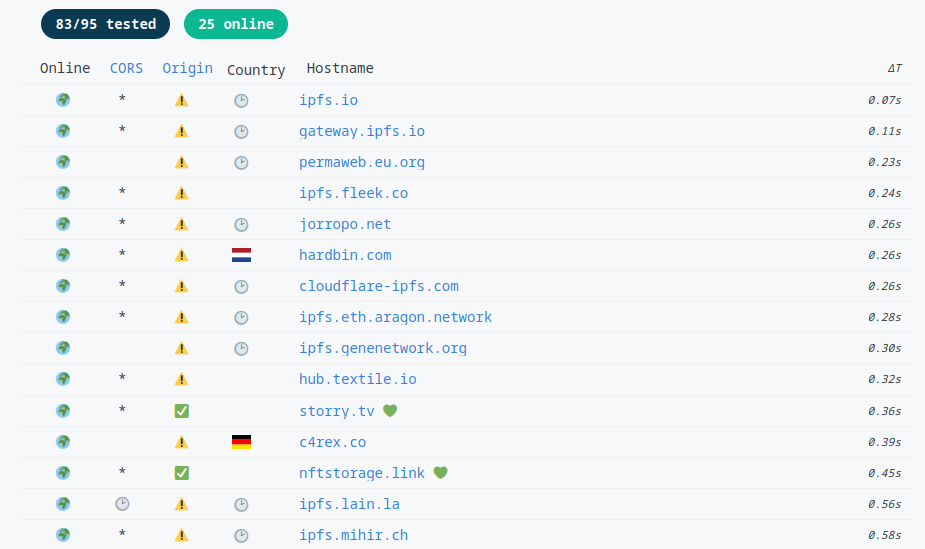
\includegraphics[width=0.7\textwidth]{Figures/ipfs_entry.png}
    \caption{Imagen de puntos de acceso de IPFS}
    \cite{web:gateways}
    \label{fg:ipfs_entry}
\end{figure}
Por simplicidad vamos a utilizar el \textit{gateway} de los creadores. \textbf{No significa que sea oficial}, eso no existe en el mundo distribuido.
\begin{quote}
    \url{https://ipfs.io/ipfs/QmXoypizjW3WknFiJnKLwHCnL72vedxjQkDDP1mXWo6uco/wiki/}
\end{quote}
De esta manera, tenemos acceso a una página de Wikipedia distribuida.
Esto también se puede aplicar al proyecto ya que Next.js de manera predeterminada, solo exporta ficheros estáticos. Esto resulta perfecto para IPFS.
\subsection{Separación de código y empaquetado}
Todas las librerías de web 3.0, están en un estado muy temprano y por ende no están optimizadas para ocupar poco espacio. Aunque nuestra página pueda estar alojada en IPFS y resulte en tiempos de respuestas más bajos, no significa que no haya que optimizar el tiempo de descarga del \textit{bundle} (paquete) de js. Para comprender mejor el problema y cómo poder aliviarlo, se va a poner un ejemplo. Next.js, aunque exporta HTML estático, es un framework que utiliza React para construir la interfaz. Más adelante, se explicará qué es React y por qué está seleccionado para este proyecto. Por ahora solo hay que saber que es un archivo de \verb|.js| que nuestro navegador tiene que ejecutar para que nuestra página pueda hacer algo útil.\\
En JavaScript, hay dos maneras de importar funcionalidad en un proyecto:\\
\textbf{Require}\\
\begin{lstlisting}
    // Este codigo no es recomendable.
    const react = require('react');
\end{lstlisting}
\noindent\rule{\textwidth}{0.4pt}
\textbf{Modules}\\
\begin{lstlisting}
    import react from 'react';
\end{lstlisting}
La diferencia principal es que require es síncrono e import es asíncrono.
Si es síncrono, cada instrucción se ejecuta una detrás de la anterior. En cambio con import, se deja cargando y se pasa a la siguiente instrucción.
Aunque los módulos están gradualmente adoptados \cite{web:canIuse} y han sido añadidos al \textit{spec} \cite{web:ecma}. A fecha de creación de este proyecto, \verb|Next.js| \cite{web:next.js} está configurado para hacer todo su código compatible con EC6, el \textit{spec} de 2015.
\begin{quote}
    Next.js supports \textbf{IE11 and all modern browsers} (Edge, Firefox, Chrome, Safari, Opera, et al) with no required configuration. \cite{web:next_supported}
\end{quote}
\begin{center}
    \begin{table}[h!]
        \begin{tabular}{p{0.3\linewidth}  p{0.6\linewidth}}
            \textbf{Modules} & \textbf{Require} \\ \hline
                \verb|import react from 'react';|
            & 
\verb|use strict';|

\verb|var _react = require('react');|
             \\
            Como vemos, nuestro import compacto y asíncrono en el spec de 2015, se convierte en un conjunto de código síncrono y extenso. & 
\verb|var _react2 = _interopRequireDefault(_react);|

\verb|function _interopRequireDefault(obj)|
\verb|{ return obj && obj.__esModule ? obj : { default: obj }; }|

\\
        \end{tabular}
        \label{tab:EC6_output}
    \end{table}
\end{center}
Esto es negativo para el rendimiento ya que si tenemos muchos \verb|require| nuestra página tardará más en ser interactiva porque está esperando a que el resto de módulos se lleguen a descargar y verificar.
Por eso mismo, Next.js \cite{web:next.js} nos permite hacer lo siguiente.
\begin{lstlisting}
    // ...
    async function foo() {
        // Libreria de ejemplo
        const Fuse = (await import('fuse.js')).default
    }
    // ...
\end{lstlisting}
Cuando se ejecute la function \verb|foo|, se descargará y validará en ese momento. Delegando el peso de descargar las librerías necesarias cuando se van a usar, hace que nuestra página sea interactiva en menos tiempo.
\subsection{Remix}
Remix es un entorno de desarrollo integrado para poder desarrollar \textit{smart contracts}. Dispone de una red de prueba, además de ser capaz de comunicarse con la cartera. De esta manera podemos hacer todas las pruebas que queramos sin tener que quemar gas por el camino. Entiéndase gas como traducción literal de quemar dinero.
Ya que nuestro entorno de desarrollo, tiene una implementación local de Ganache, que se menciona más adelante, estamos interesados en utilizar Metamask para conectarnos directamente a la red de prueba \ref{fg:remix}.
\begin{figure}[H]
    \centering
    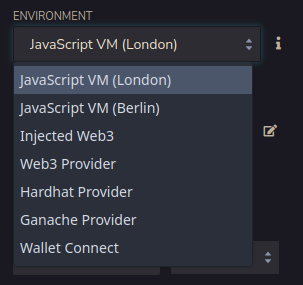
\includegraphics[width=0.4\textwidth]{Figures/remix.png}
    \caption{Posibles conexiones de Remix.}
    \cite{web:remix}
    \label{fg:remix}
\end{figure}
Metamask, de manera predeterminada, se conectara a la red principal de Ethereum e integrará una variable especial en el objeto \verb|window| de nuestro navegador.
\begin{lstlisting}
    if (typeof window.ethereum !== 'undefined') {
        console.log('Metamask is installed!');
    }
\end{lstlisting}
De la siguiente manera, se puede comprobar si Metamask está instalado.
Como desarrollador, solamente se tiene que seleccionar una dirección local para empezar.
\subsection{Ganache}
Ganache permite generar redes \textit{blockchain} locales. Metamask se puede conectar a esta red e interactuar con ella.
\begin{lstlisting}
    ganache-cli -p 8545 --mnemonic 
    \" word desert grief seven feature sight 
    object message upon lesson boat praise \" 
    --networkId 1337 --db ganache/db -q
\end{lstlisting}
Con el siguiente comando, se puede establecer un puerto con \verb|-p 8545|, se puede asegurar la carga de las mismas cuentas estableciendo un nemotécnico e introduciendo el id de la red, la cual tiene que ser 1337 ya que es local. Por ultimo, establecer una ruta para guardar todos los datos de la red. Es decir, todos los bloques de la \textit{blockchain}.
\subsection{Control de versiones}
Para este proyecto, se ha seleccionado \verb|git| como aplicación de control de versiones y GitHub \ref{fg:github} como repositorio remoto. Como este proyecto es código abierto, se ha creado un repositorio público para poder mostrar todos los pasos de desarrollo. De esa manera queda expuestos todos los \textit{commits} (confirmaciones) asociados a \textit{sprints}. Este repositorio también es útil como expositor temporal. Cualquier persona puede ver el desarrollo y verificar la integridad de nuestra solución.
\begin{figure}[h!]
    \centering
    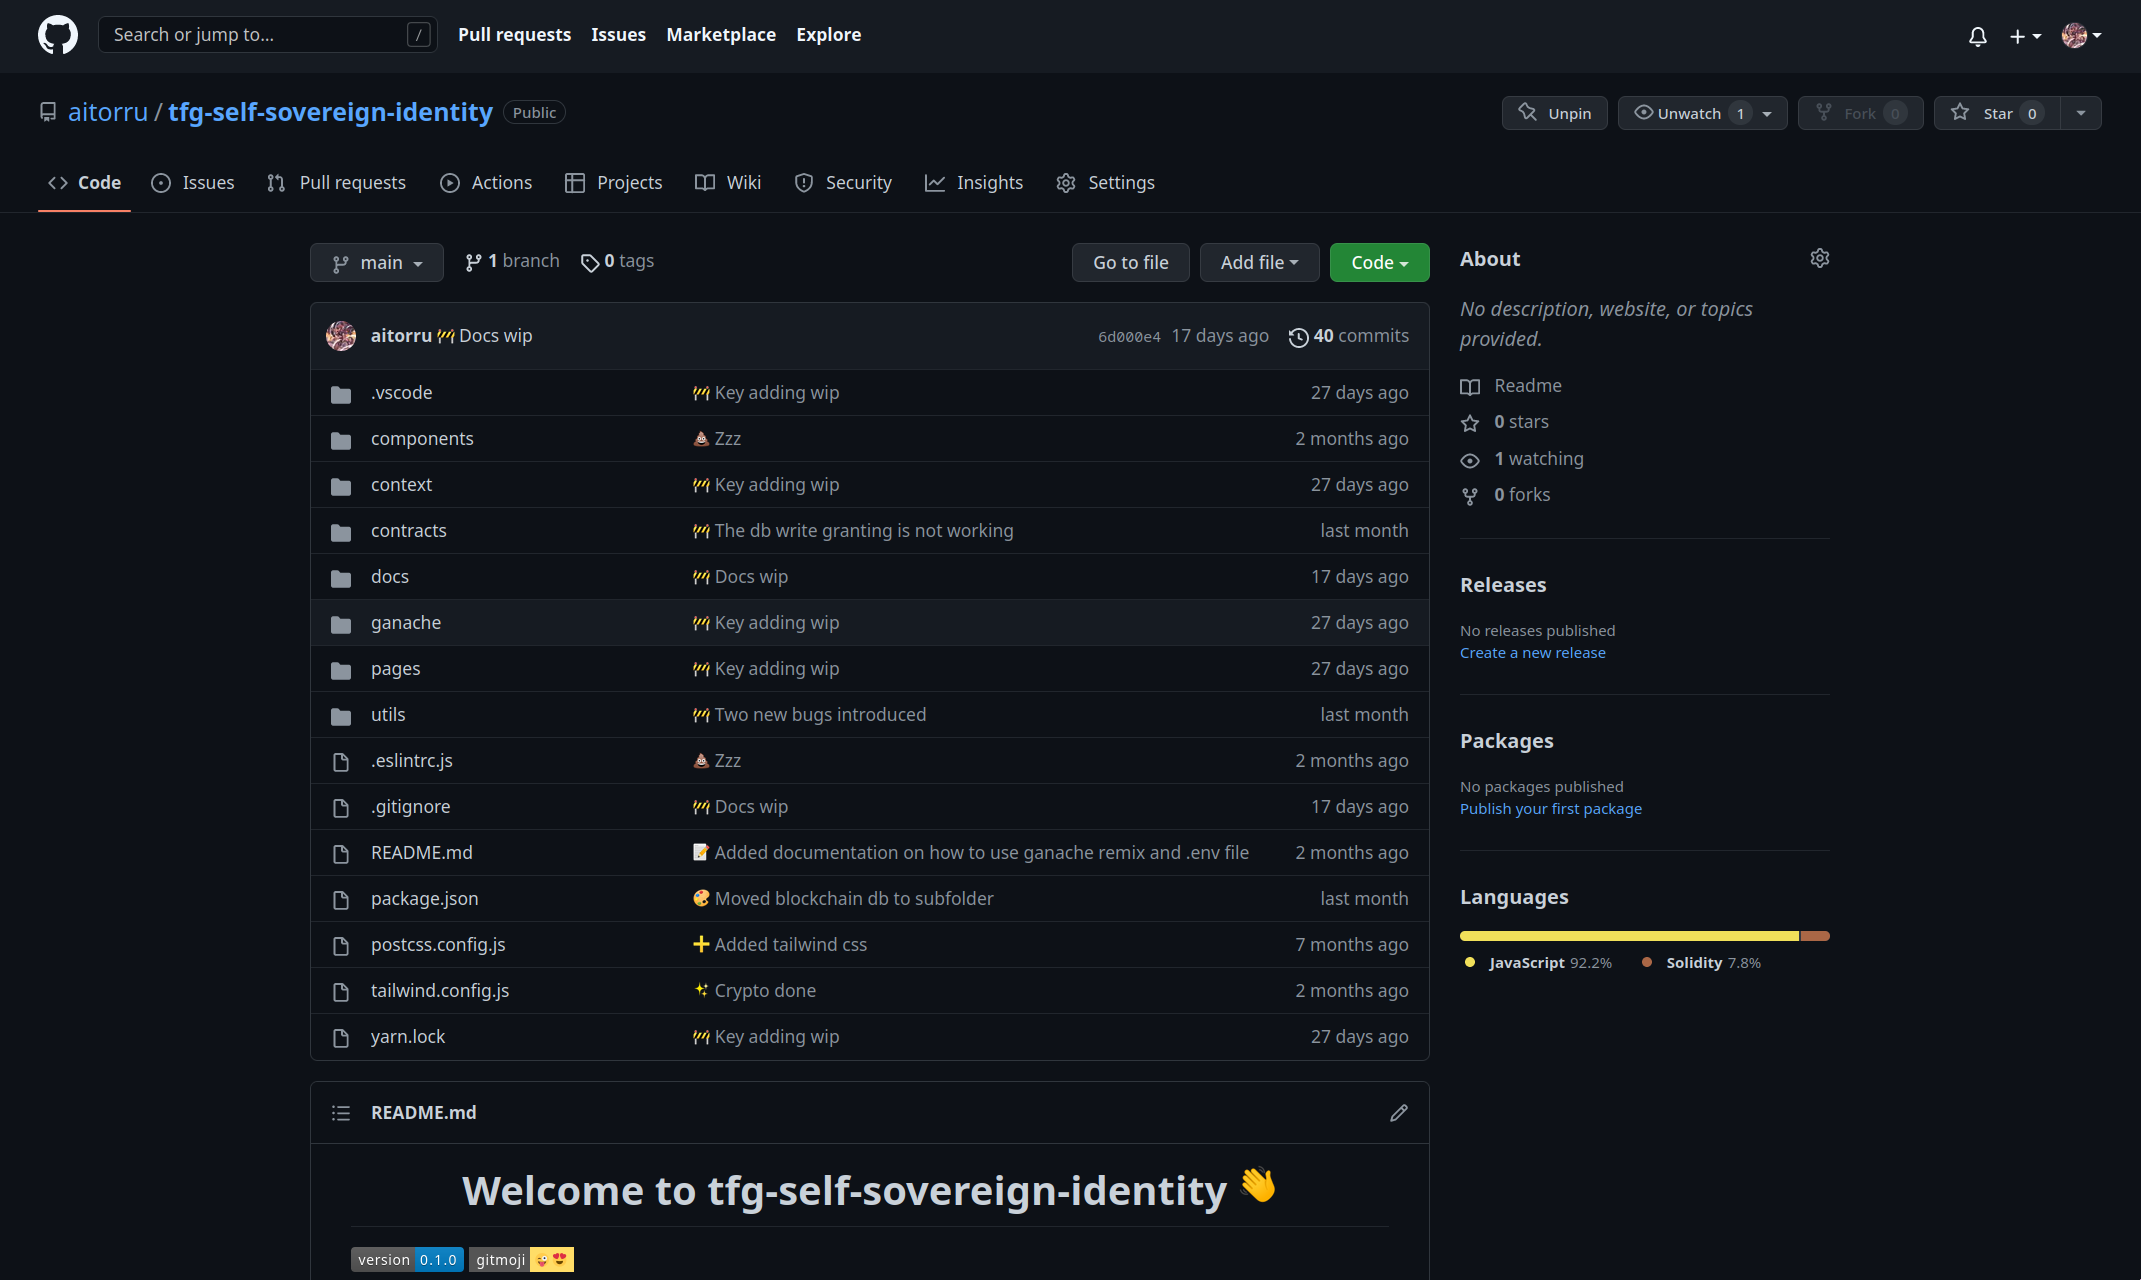
\includegraphics[width=0.8\textwidth]{Figures/github.png}
    \caption{Repositorio de github del proyecto}
    \label{fg:github}
    \cite{web:repo}
\end{figure}
\subsection{Contexto}
Para una planificación de temas, se usó una herramienta diferente. En vez de utilizar un fichero o una nota en \verb|notion.so|, se decidió utilizar apuntes en el código. Como se tenia acceso a los objetivos desde el inicio del desarrollo, se podían crear funciones vacías a modo de punto de inicio. Después se pueden crear comentarios para generar contexto.
\begin{lstlisting}
    // TODO: Hacer funcionar el proyecto
    // FIXME: El reloj no devuelve el tiempo en ISO
\end{lstlisting}
Todos los IDEs tienen la capacidad de generar árboles de \verb|TODOs| (por hacer) y \verb|FIXMEs| (arreglar). En \verb|Code - OSS| \cite{web:code-oss}, un clon de código abierto de \verb|vscode|, existen extensiones para facilitar el proyecto.
De esta manera, los comentarios \ref{fg:todoTree} sirven como herramienta de contexto a lo largo de un \textit{sprint}.
\begin{figure}[H]
    \centering
    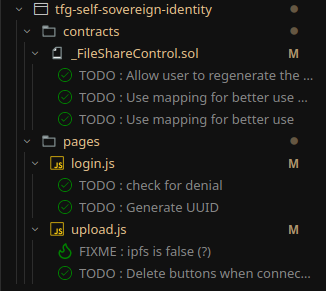
\includegraphics[width=0.5\textwidth]{Figures/TodoTree.png}
    \caption{Ejemplo de visualización de comentarios}
    \label{fg:todoTree}
\end{figure}
\section{Herramientas utilizadas}
A continuación se procederá a detallar y a analizar las herramientas utilizadas para el funcionamiento de este PFG. Las herramientas de desarrollo estarán especificadas en el apartado de metodología \ref{Metodología}.
\subsection{React}
\verb|React| es una buena opción para crear UI \textit{responsivas} y fácilmente actualizables. Como en este proyecto se están escuchando eventos de la red y actualizando todo constantemente, utilizar este \textit{framework} es una gran opción. \verb|React| nos ofrece \textit{hooks} para actualizar la interfaz del usuario. 
En los siguientes puntos del proyecto se explicará con detalle el uso de React en esta aplicación.
\subsection{Metamask}
Metamask es un \textit{wallet} (cartera) que se puede comunicar con la \textit{blockchain} de Ethereum, la cual dispone de funcionalidades de firma, encriptación y desencriptación muy útiles para este proyecto. Existe como una extensión en el navegador y también tiene la capacidad de usarse desde el dispositivo móvil.
\subsection{OrbitDB}
OrbitDB es una base de datos distribuida. Ha sido construida por encima de \verb|js-ipfs| (una librería que convierte nuestro navegador en un nodo de IPFS). Utiliza su sistema de \textit{peers} para poder compartir datos utilizando una ruta a la que se puede acceder. Gracias a la criptografía, se pueden implementar permisos de lectura y escritura. La información de la base de datos se guarda en el \verb|local storage| del navegador. El funcionamiento es totalmente nuevo dentro de los paradigmas actuales, principalmente por la naturaleza inmutable de IPFS. La dirección de una base de datos hace referencia a un fichero en IPFS.\\
\verb|/OrbitDB/Qmd8TmZrWASypEp4Er9tgWP4kCNQnW4ncSnvjvyHQ3EVSU/database-name|\\
Esta URL contiene las siguientes partes.
\begin{itemize}
    \item \textbf{OrbitDB}: hace referencia a que el fichero existe en una carpeta llamada OrbitDB. Esto se hace por simplicidad. Todos los proyectos introducen sus datos bajo las carpetas de su organización para poder saber a quien pertenecen.
    \item \textbf{Qmd8TmZrWASypEp4Er9tgWP4kCNQnW4ncSnvjvyHQ3EVSU}: esta sección es generada aleatoriamente, sobre todo para evitar conflictos. Esto genera un problema, ya que al ser aleatorio no podemos saber cual es la base de datos de nuestro del \textit{peer} al que queremos contactar. Este problema se solucionará más adelante en el proyecto.
    \item \textbf{database-name}: este último apartado es libre. Esto significa que como ya hemos evitado conflictos entre bases de datos, se puede aportar un nombre útil para la aplicación. En el caso de este proyecto, se utiliza la dirección de la \textit{wallet} del usuario.
\end{itemize}
En esta dirección hay un archivo que solamente tiene la clave publica de OrbitDB. De este modo, todos los usuarios que se quieran conectar pueden leer la clave con la seguridad de que no ha sido manipulada.
\begin{figure}[H]
    \centering
    \includegraphics[width=0.7\textwidth]{Figures/OrbitDB.png}
    \caption[Diagrama básico de conexión de OrbitDB]{Diagrama que ejemplifica una base de datos compartida en el que el nodo propietario es el verde.}
    \label{fg:orbit}
\end{figure}
En el siguiente escenario \ref{fg:orbit}, hay una serie de nodos escuchando al nodo con la clave pública que han podido obtener del fichero. Al mismo tiempo, todos escuchan al mismo \textit{topic} que han obtenido desde el fichero.
\begin{figure}[h!]
    \centering
    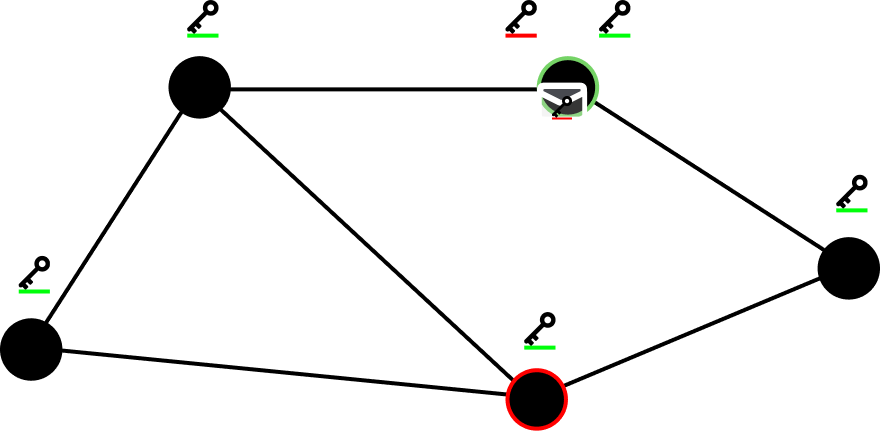
\includegraphics[width=0.7\textwidth]{Figures/Message sent.png}
    \caption{El nodo verde envía un mensaje.}
    \label{fg:messageSent}
\end{figure}
\begin{figure}[h!]
    \centering
    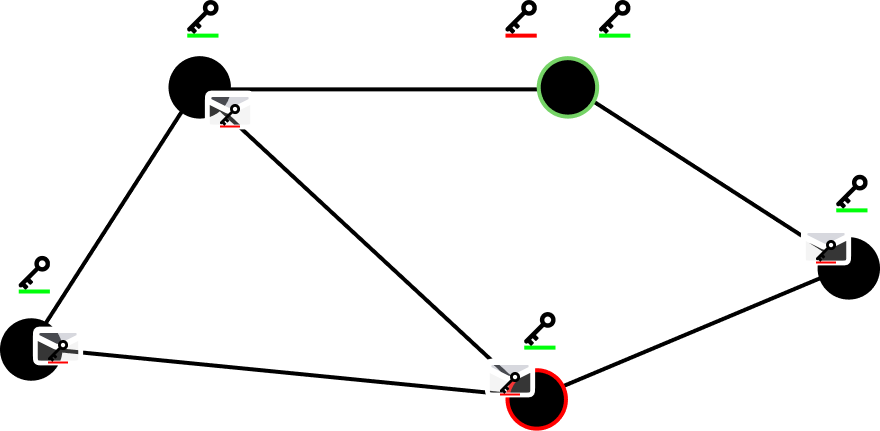
\includegraphics[width=0.7\textwidth]{Figures/Message arived.png}
    \caption{El resto de la red recibe el mensaje}
    \label{fg:messageRecived}
\end{figure}
Los mensajes salen del \textit{host} verde firmados con su clave privada \ref{fg:messageSent}. Utilizando la clave publica del \textit{host} verde (que han obtenido de la dirección original de IPFS) pueden verificar la legitimidad del origen y actualizar su copia de la base de datos \ref{fg:messageRecived}.
\begin{figure}[h!]
    \centering
    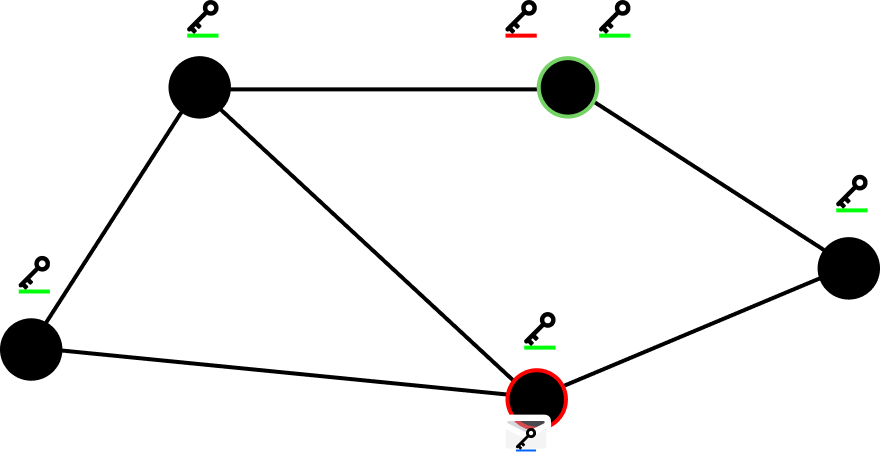
\includegraphics[width=0.7\textwidth]{Figures/Message is compromissed.png}
    \caption{El nodo rojo intenta sobrescribir la información de los nodos}
    \label{fg:messageSentRed}
\end{figure}
\begin{figure}[h!]
    \centering
    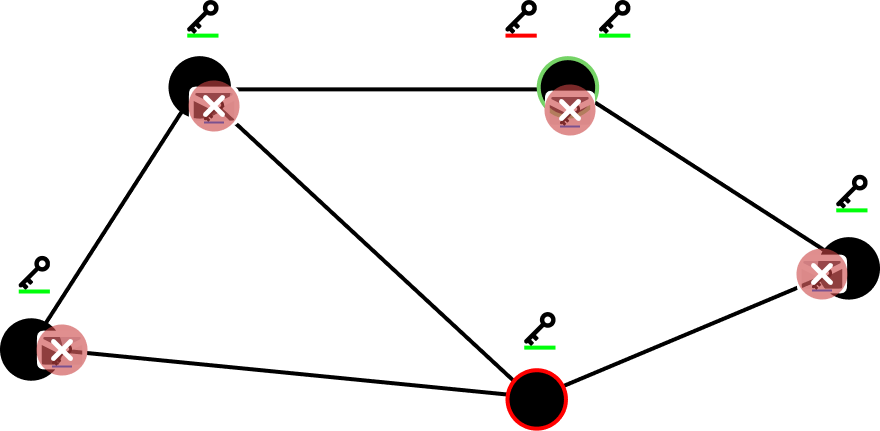
\includegraphics[width=0.7\textwidth]{Figures/Message rejected.png}
    \caption{El resto de la red rechaza el mensaje, ya que la clave no se puede verificar}
\end{figure}
\newpage
\thispagestyle{empty}